\documentclass{article}
\usepackage[utf8]{inputenc}
\usepackage{geometry}
\usepackage{fullpage}
\usepackage{ctex}
\usepackage{float}
\usepackage{graphicx}
\usepackage{subfigure}

\title{Colorization using Optimization}
\author{王世因 2016011246}
\date{}
\begin{document}
\maketitle

\tableofcontents
\newpage

\section{算法简介}
在YIQ和YUV图片格式中,Y代表图片的亮度,含有各种阴影细节,单独输出后就可以得到黑白照片。


\section{图片上色}

\begin{figure}[H]
\centering
\subfigure{
\begin{minipage}[t]{0.3\linewidth}
\centering
\includegraphics[width=\linewidth]{gray_0.png}
\caption{gray}
\end{minipage}%
}%
\subfigure{
\begin{minipage}[t]{0.3\linewidth}
\centering
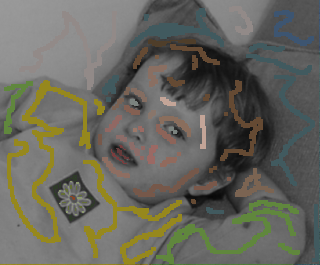
\includegraphics[width=\linewidth]{sketch_0.png}
\caption{sketch}
\end{minipage}%
}%
\subfigure{
\begin{minipage}[t]{0.3\linewidth}
\centering
\includegraphics[width=\linewidth]{result_0.png}
\caption{result}
\end{minipage}
}%
\centering
\end{figure}



\begin{figure}[H]
\centering
\subfigure{
\begin{minipage}[t]{0.3\linewidth}
\centering
\includegraphics[width=\linewidth]{gray_5.png}
\caption{gray}
\end{minipage}%
}%
\subfigure{
\begin{minipage}[t]{0.3\linewidth}
\centering
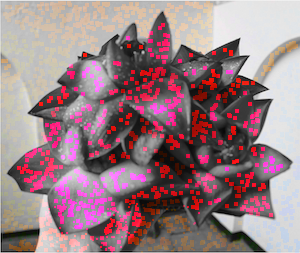
\includegraphics[width=\linewidth]{sketch_5.png}
\caption{sketch}
\end{minipage}%
}%
\subfigure{
\begin{minipage}[t]{0.3\linewidth}
\centering
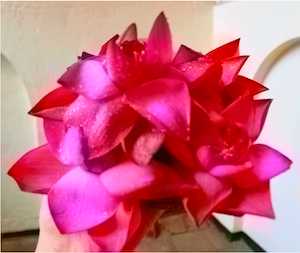
\includegraphics[width=\linewidth]{result_5.png}
\caption{result}
\end{minipage}
}%
\centering
\end{figure}

\section{从静态图片扩展到视频}
\subsection{准静态图片的像素采样法}
这部分算法对应代码文件$video\_color.py$,我通过在上一帧图片中获得一些采样点来,作为本帧的标注色彩。因为我采用的是30帧一秒的视频质量,视频中相邻两帧间的变化不大,所以可以直接进行一定的色彩继承分析。因为优化算法最小化的是总体的灰度匹配概率,因为部位微小位移造成的标注误差可以在最优化求解的时候被补偿。相比下面的这种方法,本方法因为没有增加权重矩阵的大小,所以计算起来更快,占用的计算资源也更小。

\begin{figure}[H]
\centering
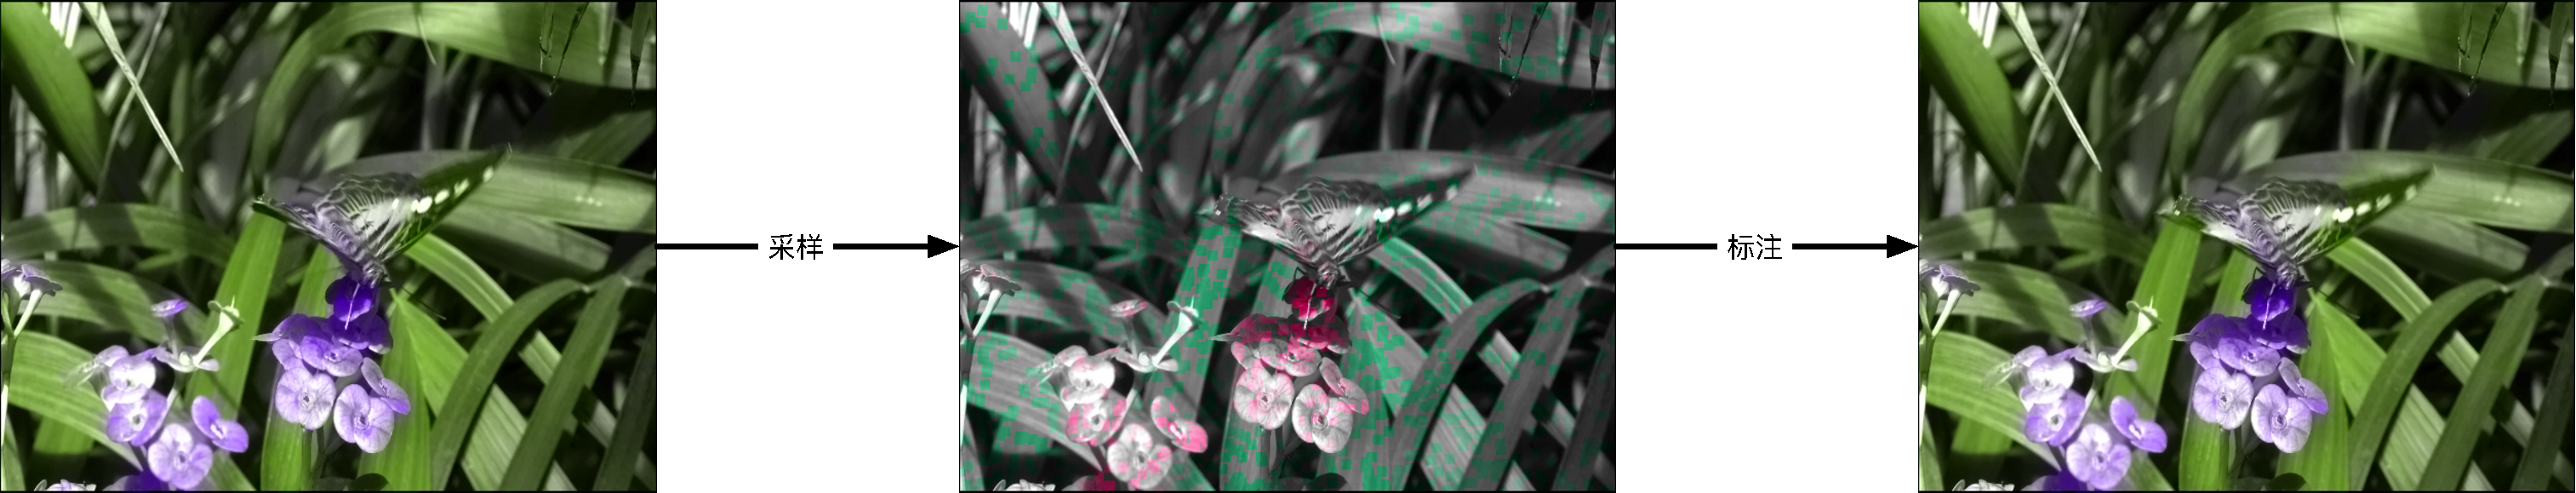
\includegraphics[scale=0.3]{seq.pdf}
\caption{相邻帧之间采样标注色彩}
\end{figure}

\subsection{位移捕捉和临点检测}
这是原文中提到的方法,通过算法Lucas-Kanade计算各个像素点的运动情况,找到相邻两帧中对应的点,拓展静态图片中像素点的临点,再进行求解。
\begin{equation}
Y_t(p) +  \nabla Y_{(x, y)} v = 0
\end{equation}

\begin{equation}
\left[
\begin{array}{cc}
Y_x(p_1) & Y_y(p_1)\\
Y_x(p_2) & Y_y(p_2)\\
Y_x(p_3) & Y_y(p_3)\\
\ldots & \ldots \\
Y_x(p_{25}) & Y_y(p_{25})\\
\end{array}
\right]
\left[
\begin{array}{c}
v_x\\
v_y
\end{array}
\right]
= - 
\left[
\begin{array}{c}
Y_t(p_1)\\
Y_t(p_2)\\
Y_t(p_3)\\
\ldots\\
Y_t(p_{25})\\
\end{array}
\right]
\end{equation}

\begin{equation}
||(x_{t+1}-v_x, y_{t+1}-v_y) - (x_t, v_t)||< T
\end{equation}

在具体的实现上,我根据上面的公式生成一个包含两帧的权重矩阵,重新跑一边静态图片的上色算法,得到后一帧的色彩。因为权重矩阵是一个很大的稀疏矩阵,这个做法的权重矩阵是静态图片权重矩阵的四倍,显著地增加了耗时。对比来看,这个方法适用于移动迅速的图片和每秒帧数少的图片。相应的代码实现在$video\_dynamic.py$中,对应$frame.DynamicFrame$类。

\section{算法的不足}


\end{document}